


\chapter{Implementacija i korisničko sučelje}
		
		
\section{Korištene tehnologije i alati}

	\textbf{\textit{dio 2. revizije}}
	
	 \textit{Detaljno navesti sve tehnologije i alate koji su primijenjeni pri izradi dokumentacije i aplikacije. Ukratko ih opisati, te navesti njihovo značenje i mjesto primjene. Za svaki navedeni alat i tehnologiju je potrebno \textbf{navesti internet poveznicu} gdje se mogu preuzeti ili više saznati o njima}.
	
	
	\eject 


\section{Ispitivanje programskog rješenja}
	
	\textbf{\textit{dio 2. revizije}}\\
	
	 \textit{U ovom poglavlju je potrebno opisati provedbu ispitivanja implementiranih funkcionalnosti na razini komponenti i na razini cijelog sustava s prikazom odabranih ispitnih slučajeva. Studenti trebaju ispitati temeljnu funkcionalnost i rubne uvjete.}

	
	\subsection{Ispitivanje komponenti}
	\textit{Potrebno je provesti ispitivanje jedinica (engl. unit testing) nad razredima koji implementiraju temeljne funkcionalnosti. Razraditi \textbf{minimalno 6 ispitnih slučajeva} u kojima će se ispitati redovni slučajevi, rubni uvjeti te izazivanje pogreške (engl. exception throwing). Poželjno je stvoriti i ispitni slučaj koji koristi funkcionalnosti koje nisu implementirane. Potrebno je priložiti izvorni kôd svih ispitnih slučajeva te prikaz rezultata izvođenja ispita u razvojnom okruženju (prolaz/pad ispita). }
	
	
	
	\subsection{Ispitivanje sustava}
	
	 \textit{Potrebno je provesti i opisati ispitivanje sustava koristeći radni okvir Selenium\footnote{\url{https://www.seleniumhq.org/}}. Razraditi \textbf{minimalno 4 ispitna slučaja} u kojima će se ispitati redovni slučajevi, rubni uvjeti te poziv funkcionalnosti koja nije implementirana/izaziva pogrešku kako bi se vidjelo na koji način sustav reagira kada nešto nije u potpunosti ostvareno. Ispitni slučaj se treba sastojati od ulaza (npr. korisničko ime i lozinka), očekivanog izlaza ili rezultata, koraka ispitivanja i dobivenog izlaza ili rezultata.\\ }
	 
	 \textit{Izradu ispitnih slučajeva pomoću radnog okvira Selenium moguće je provesti pomoću jednog od sljedeća dva alata:}
	 \begin{itemize}
		 \item \textit{dodatak za preglednik \textbf{Selenium IDE} - snimanje korisnikovih akcija radi automatskog ponavljanja ispita	}
		 \item \textit{\textbf{Selenium WebDriver} - podrška za pisanje ispita u jezicima Java, C\#, PHP koristeći posebno programsko sučelje.}
	 \end{itemize}
	 \textit{Detalji o korištenju alata Selenium bit će prikazani na posebnom predavanju tijekom semestra.}
	
	\eject 


\section{Dijagram razmještaja}
	
	\textbf{\textit{dio 2. revizije}}
	
	 \textit{Potrebno je umetnuti \textbf{specifikacijski} dijagram razmještaja i opisati ga. Moguće je umjesto specifikacijskog dijagrama razmještaja umetnuti dijagram razmještaja instanci, pod uvjetom da taj dijagram bolje opisuje neki važniji dio sustava.}
	
	\eject 

\section{Upute za puštanje u pogon}

		
		\textbf{Prijava u Azure račun}
		
	   \noindent Korisnik se treba prijaviti u svoj Microsoft Azure račun.
		
		\vspace{10mm}
		
		\noindent\textbf{Stvaranje baze podataka na Azure serveru}

		\noindent Nakon prijave, korisnik treba u izborniku odabrati opciju "Create a resource", te od ponuđenih odabrati "SQL Database".

		\vspace{10mm}
	
		\begin{figure}[H]
			 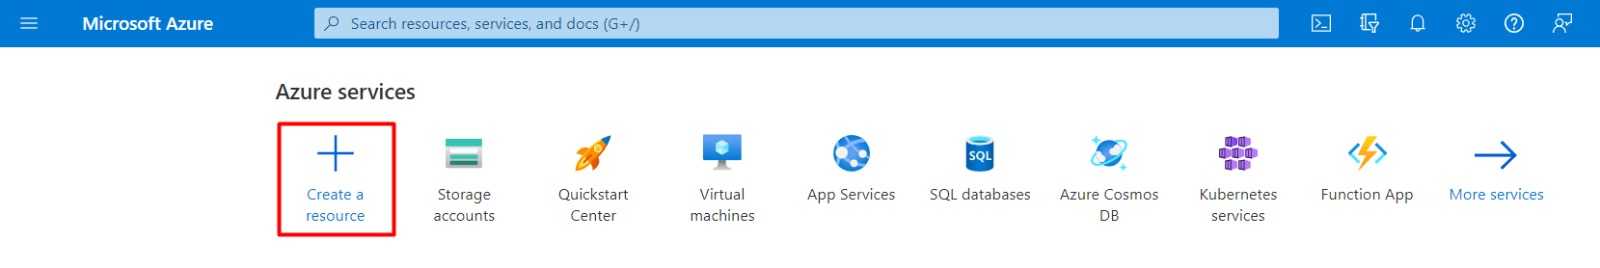
\includegraphics[width=\linewidth]{./slike/baza0.jpg}
			  \centering
			  \caption{Odabir opcije "Create a resource"}
		  \end{figure}

		\vspace{20mm}
		
	
		\begin{figure}[H]
			 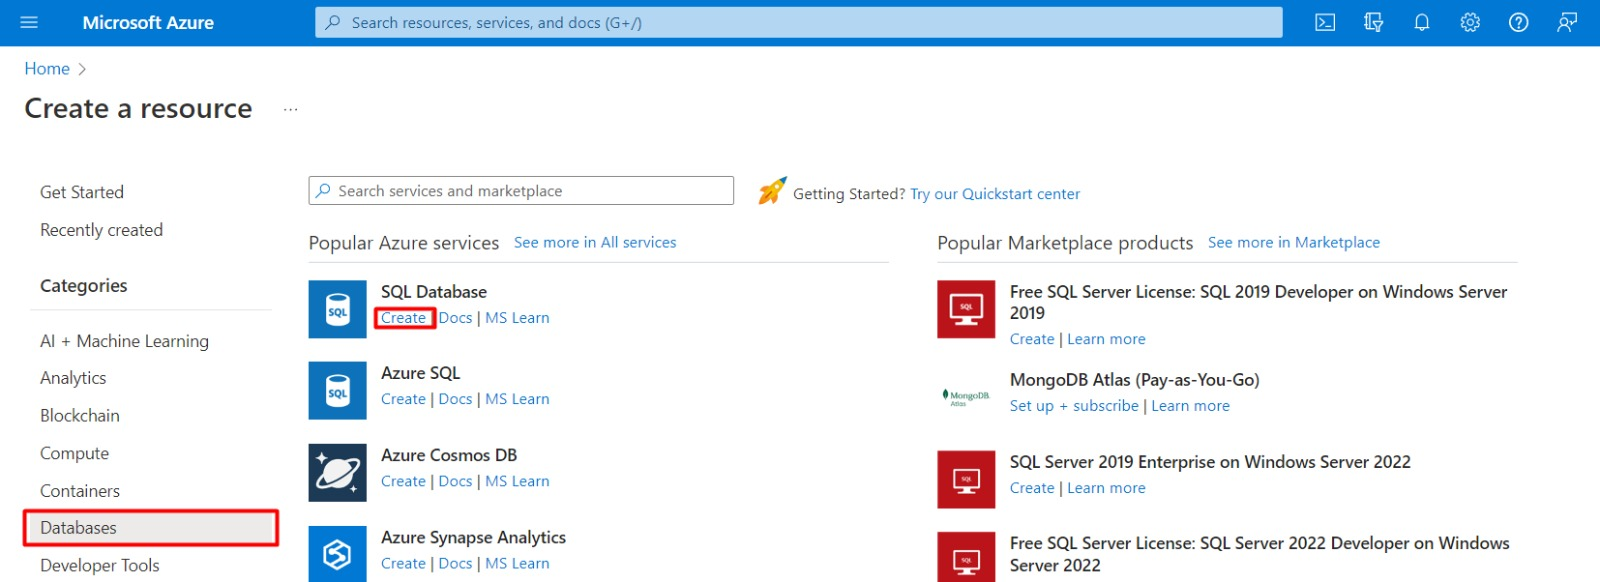
\includegraphics[width=\linewidth]{./slike/baza1.jpg}
			  \centering
			  \caption{Odabir opcije "SQL Database"}
		  \end{figure}
		  
	
	\vspace{25mm}

	   \noindent Korisnik treba dati ime bazi, napraviti njezin resource group i server. Također potrebno je odabrati i pricing tier, odnosno cjenovni rang koji ovisi o željenim performansama.
	
		\vspace{10mm}

		\begin{figure}[H]
			 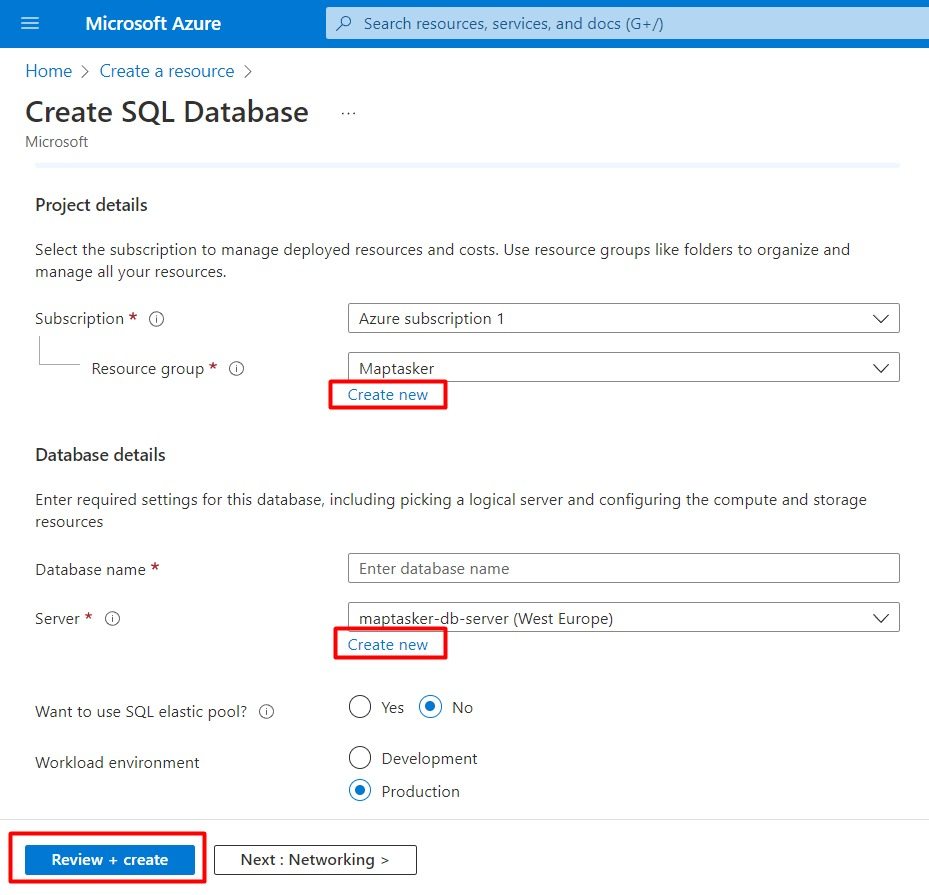
\includegraphics[width=\linewidth]{./slike/baza2.jpg}
			  \centering
			  \caption{Dodavanje željenih svojstava bazi}
		  \end{figure}

		
		\vspace{5mm}

		\noindent Potrebno je otvoriti Azure Data Studio i spojiti se na lokalni server, zatim desnim klikom na lokalnu bazu na padajućem izborniku odabrati opciju "Data-tier Application Wizard". Nakon toga korisnik treba označiti zadnju navedenu operaciju ("Export the schema..." ), kliknuti Next, te na kraju odabrati lokaciju kreirane .bacpac datoteke i pričekati dok se datoteka ne stvori.


		\vspace{10mm}

		\begin{figure}[H]
			 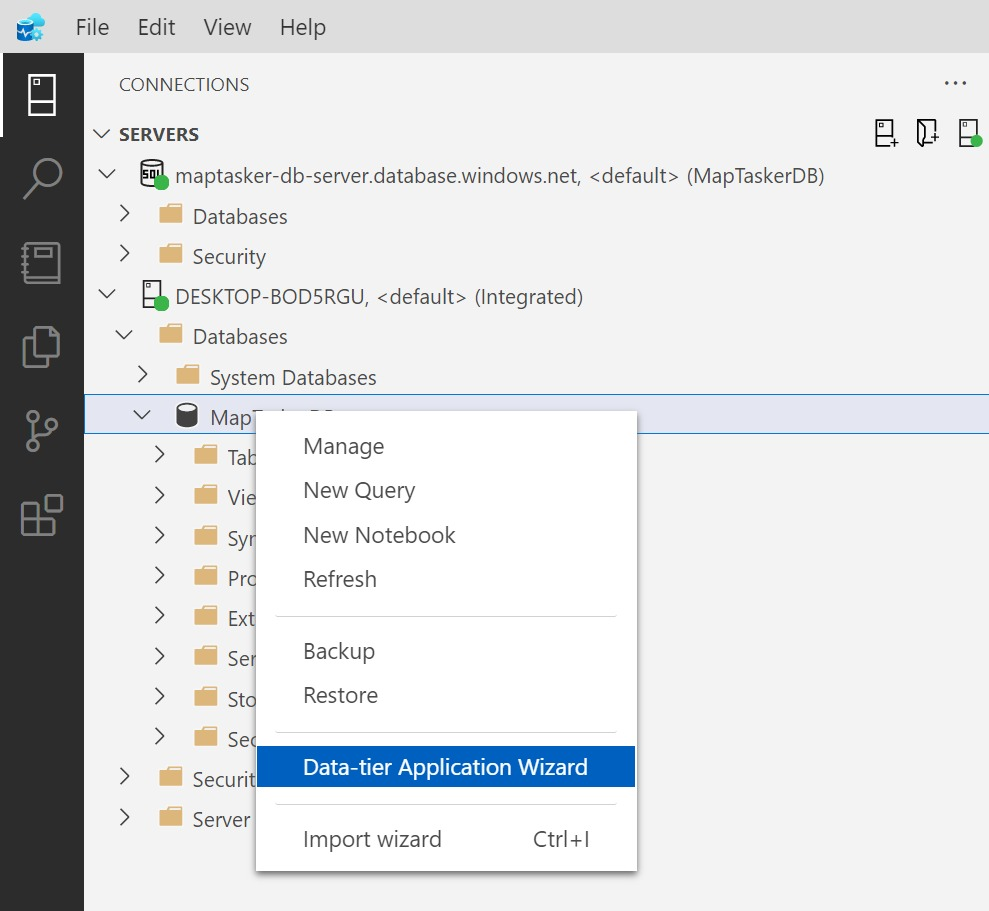
\includegraphics[width=\linewidth]{./slike/baza3.jpg}
			  \centering
			  \caption{Odabir opcije "Data-tier Application Wizard"}
		  \end{figure}

		\vspace{25mm}

		\begin{figure}[H]
			 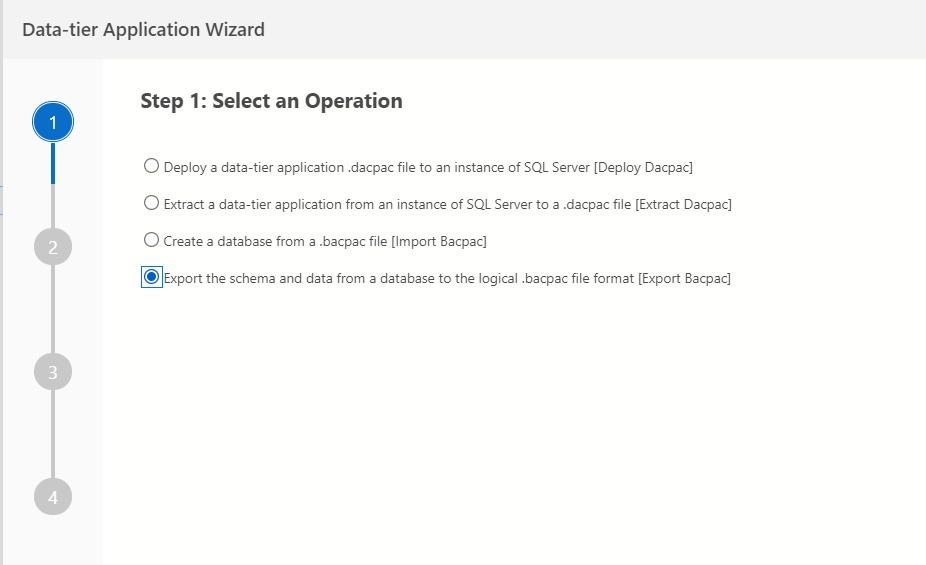
\includegraphics[width=\linewidth]{./slike/baza4.jpg}
			  \centering
			  \caption{Odabir željene operacije}
		  \end{figure}
		
		\vspace{15mm}

		\noindent Na kraju je potrebno spojiti se na Azure server i ponovno otvoriti "Data-tier Application Wizard". Zatim korisnik treba odabrati opciju "Create a database" kojom će stvoriti bazu, pratiti daljne korake i odabrati prethodno stvoreni .bacpac file.

		\vspace{10mm}

		\begin{figure}[H]
			 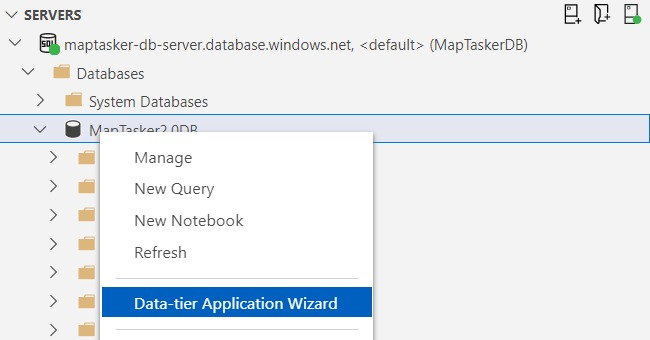
\includegraphics[width=\linewidth]{./slike/baza5.jpg}
			  \centering
			  \caption{Odabir opcije "Data-tier Application Wizard"}
		  \end{figure}

		\vspace{10mm}

		\begin{figure}[H]
			 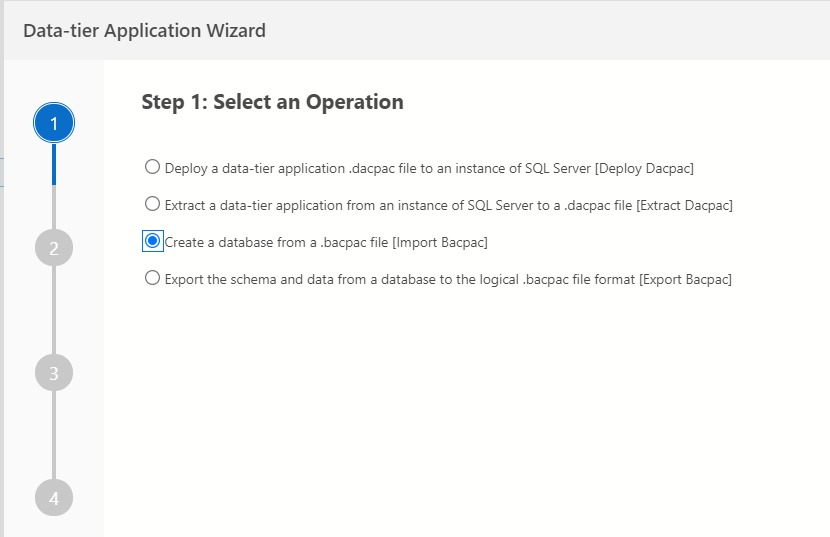
\includegraphics[width=\linewidth]{./slike/baza6.jpg}
			  \centering
			  \caption{Odabir operacije stvaranja baze}
		  \end{figure}

		\noindent\textbf{Stvaranje backend API-ja na Azure serveru}

		\noindent Za početak, potrebno je otvoriti projekt u Visual Studiu, i desnim klikom na Backend projekt u padajućem izborniku odabrati opciju "Publish". Zatim se preko grafičkog sučelja ulogirati u Azure i označiti isti resource group kao i za bazu.

		\vspace{10mm}

		\begin{figure}[H]
			 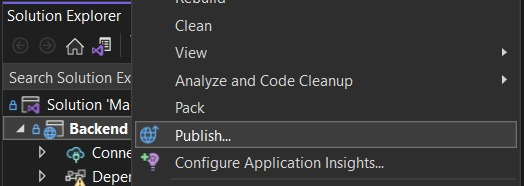
\includegraphics[width=\linewidth]{./slike/backend1.jpg}
			  \centering
			  \caption{Odabir opcije "Publish"}
		  \end{figure}
		  
		\vspace{10mm}

		\noindent Za ispravno pokretanje backenda, potrebno je otići u Azure na novonastali App Service u Configuration sučelje. Potrebno je dodati novi Application Setting naziva CONNECTION\_STRING i vrijednosti connection stringa dobivenog iz Azure postavka za bazu. Ponoviti postupak umetanja connection stringa za podizbornik Connection String, ovoga puta s nazivom ConnectionString. 

		\vspace{10mm}

		\begin{figure}[H]
			 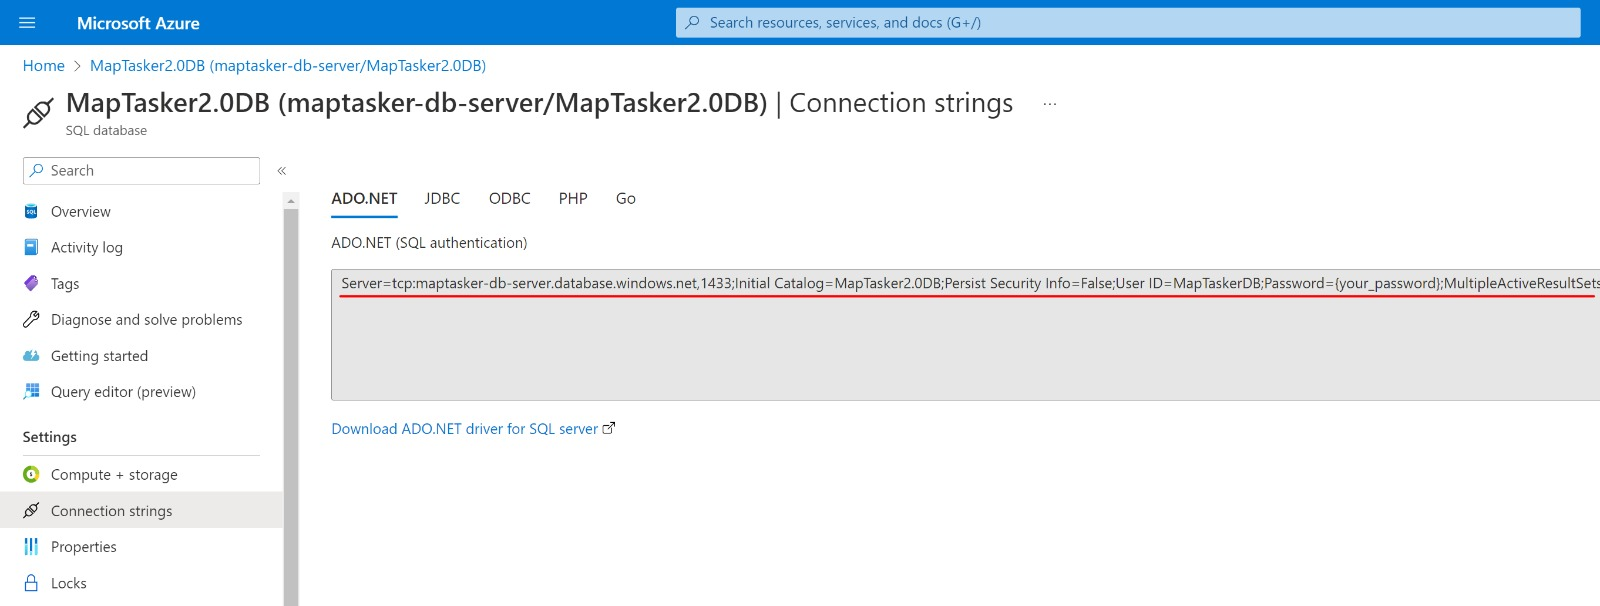
\includegraphics[width=\linewidth]{./slike/backend1a.jpg}
			  \centering
			  \caption{Lokacija vrijednosti connection stringa}
		  \end{figure}
		  
		\vspace{20mm}

		\begin{figure}[H]
			 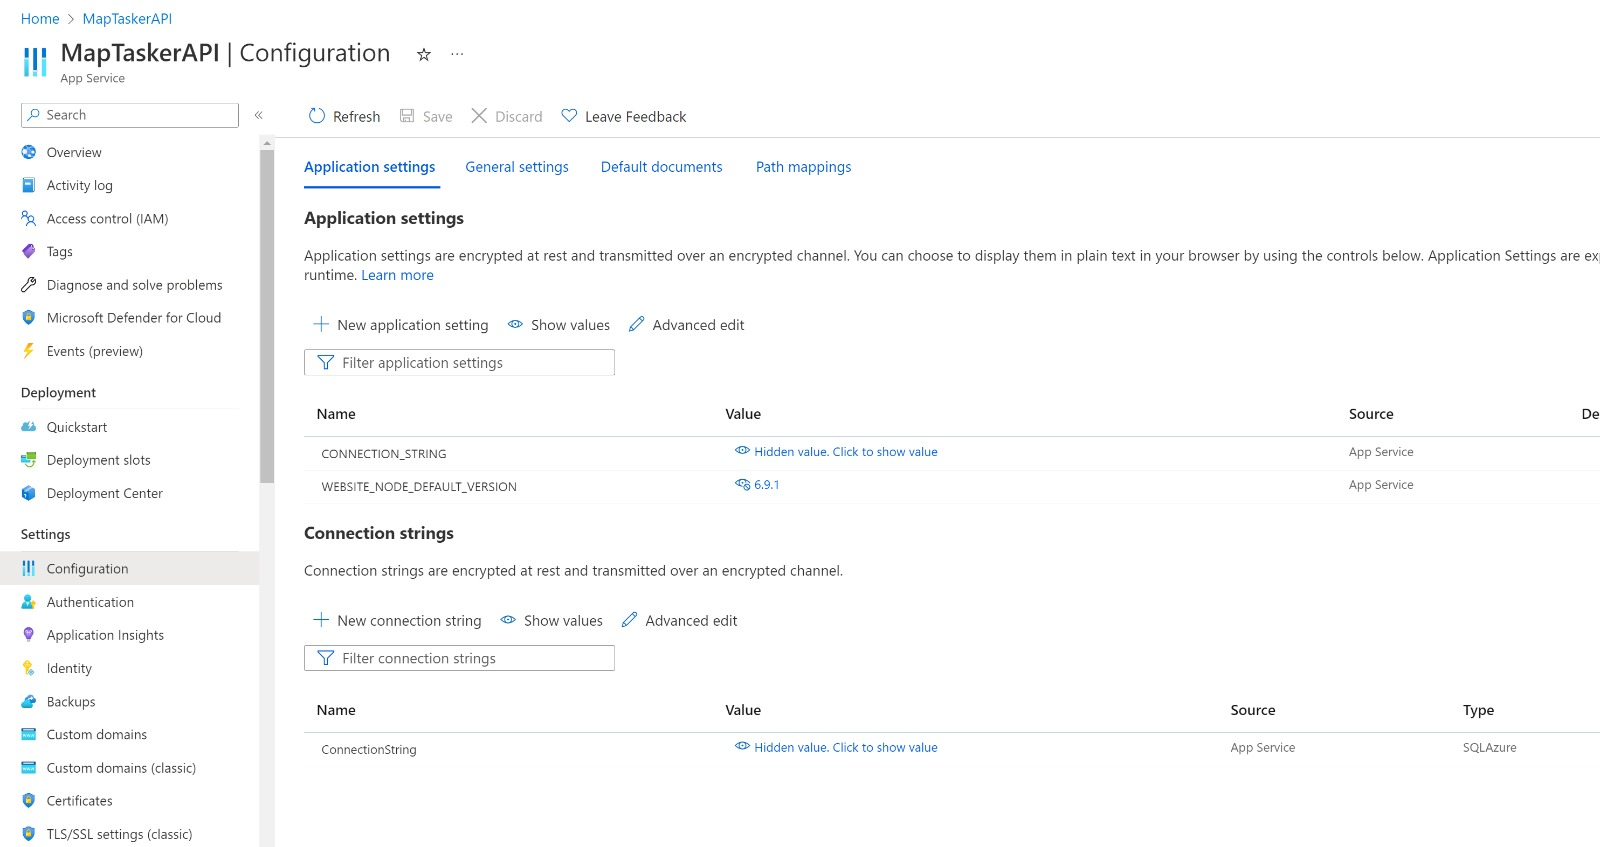
\includegraphics[width=\linewidth]{./slike/backend2.jpg}
			  \centering
			  \caption{Unos vrijednosti connection stringa}
		  \end{figure}
		
		\vspace{30mm}

		\noindent\textbf{Stvaranje frontenda aplikacije na Vercel platformi}

		\noindent Za početak nužno je uvesti git repozitorij projekta.

		\vspace{10mm}

		\begin{figure}[H]
			 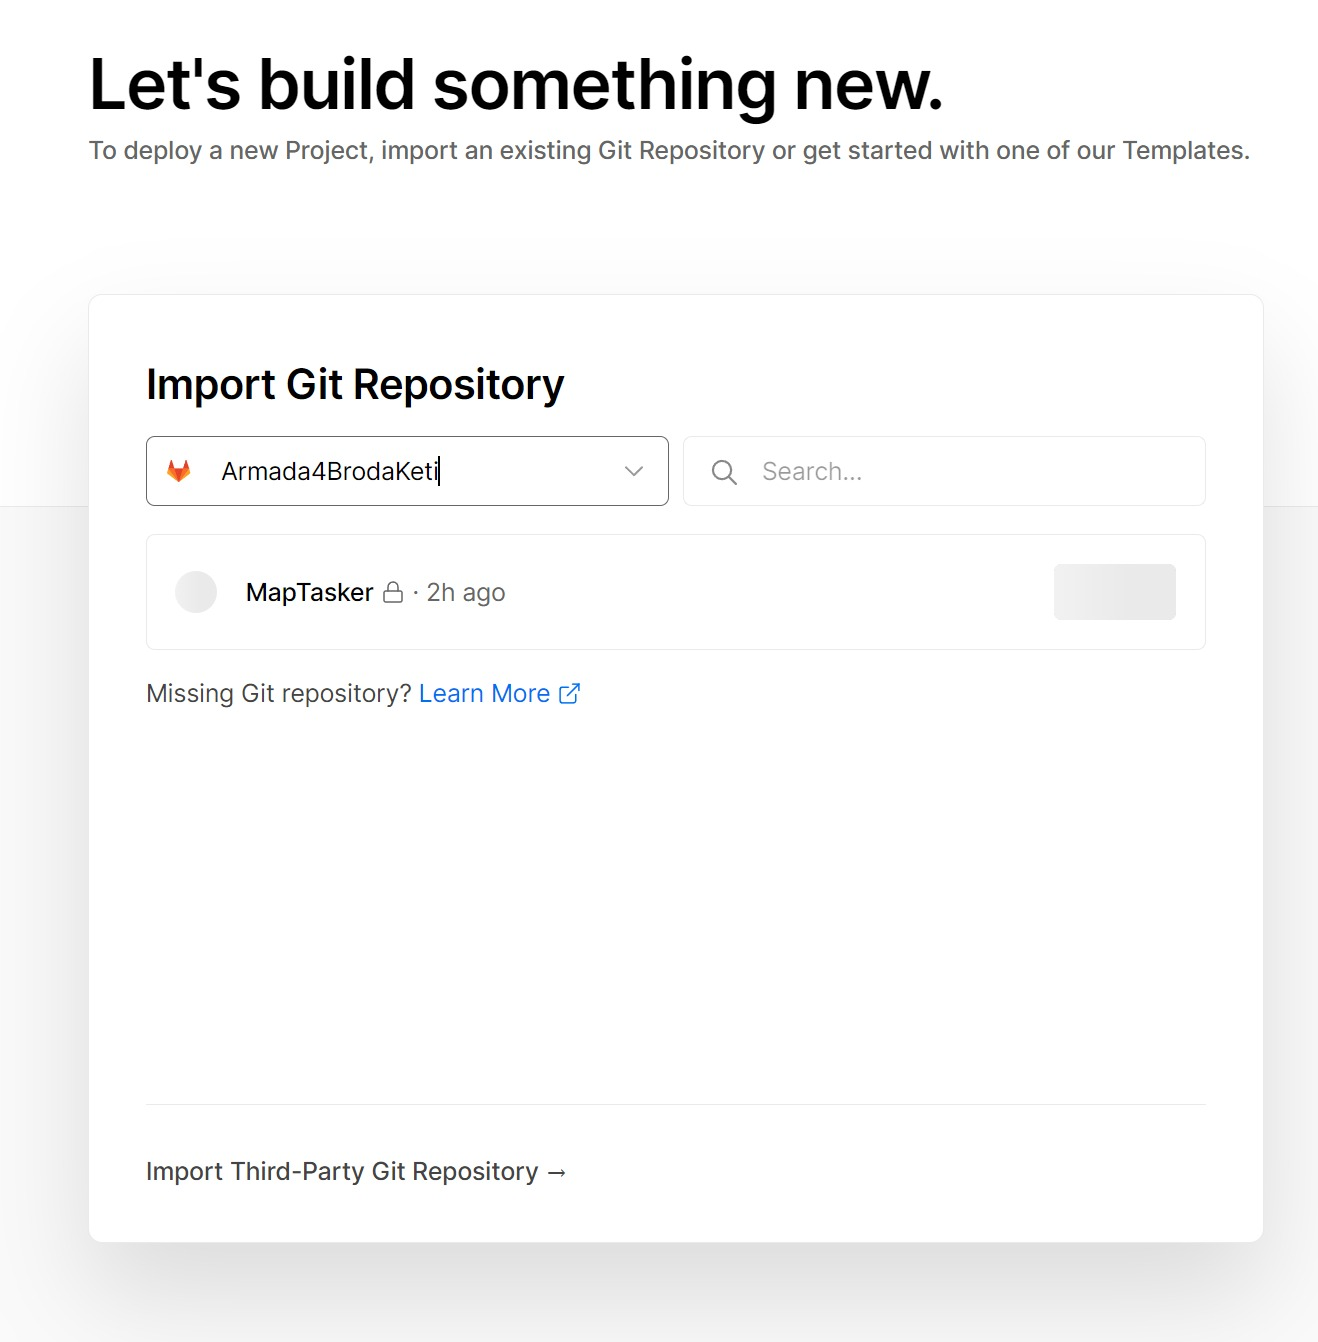
\includegraphics[width=\linewidth]{./slike/front1.jpg}
			  \centering
			  \caption{Uvoz git repozitorija projekta}
		  \end{figure}

		\vspace{20mm}

		\noindent Nakon toga potrebno je otići u "Build \& Development Settings" sučelje i postaviti naredbe potrebne za pokretanje npm skripti koje su prikazane na slici 5.12.

		\vspace{10mm}

		\begin{figure}[H]
			 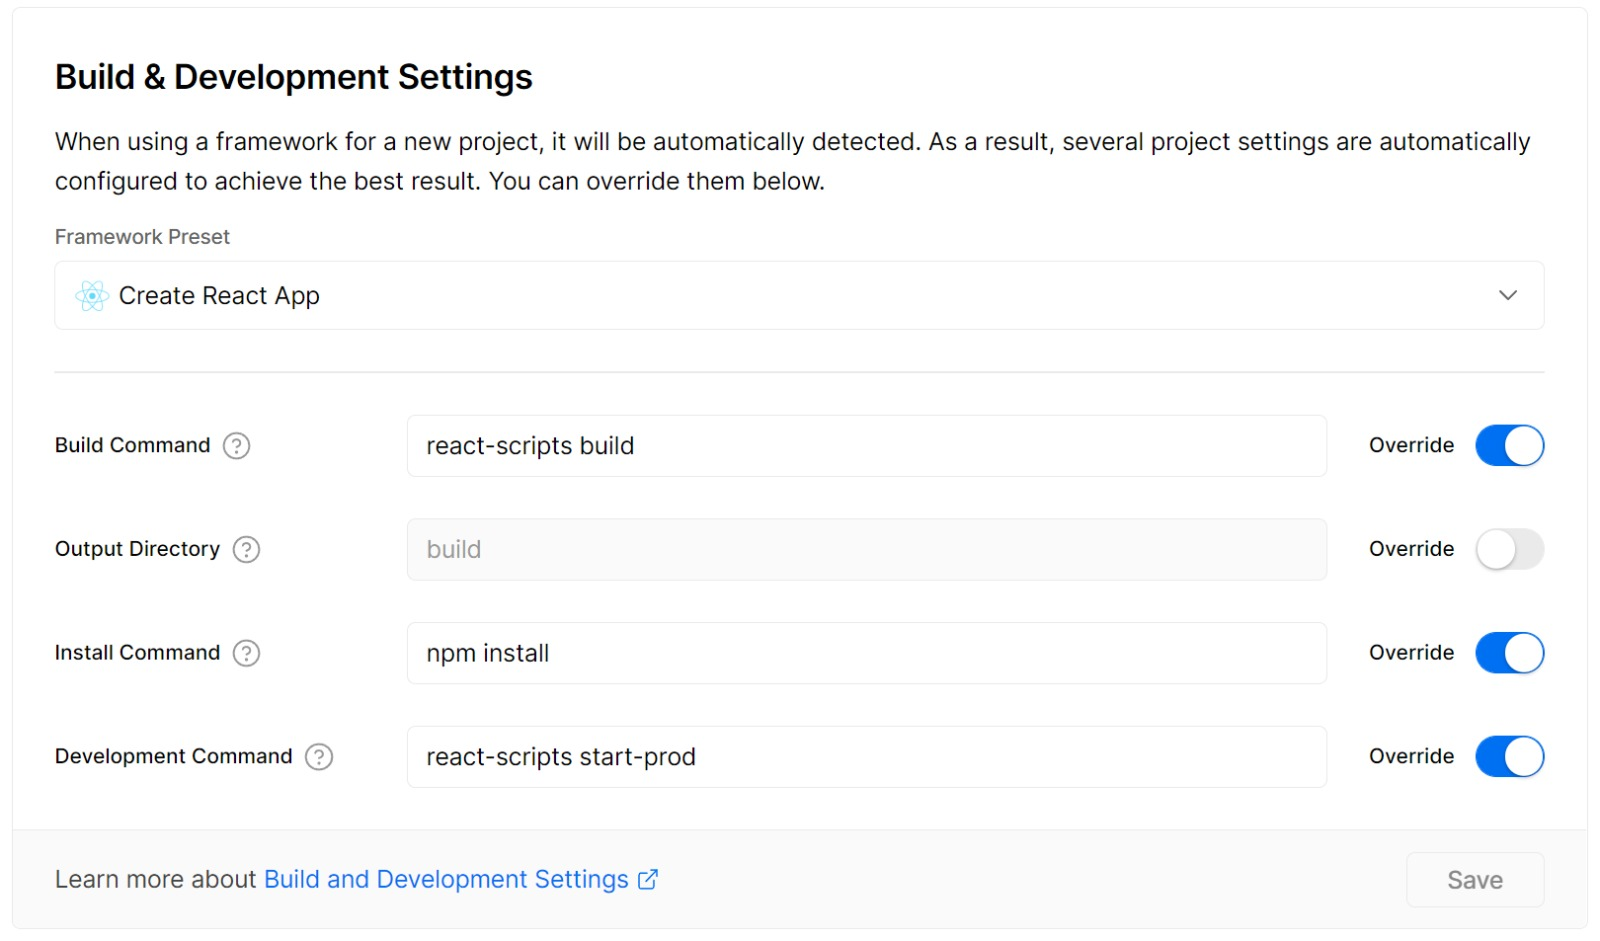
\includegraphics[width=\linewidth]{./slike/front2.jpg}
			  \centering
			  \caption{Naredbe za pokretanje npm skripti}
		  \end{figure}

		\vspace{20mm}

		\noindent U sučelju "Environment Variables" kopirati link na backend API (vidljiv u Azureu) pod ključem REACT\_APP\_API\_URL.

		\vspace{10mm}

		\begin{figure}[H]
			 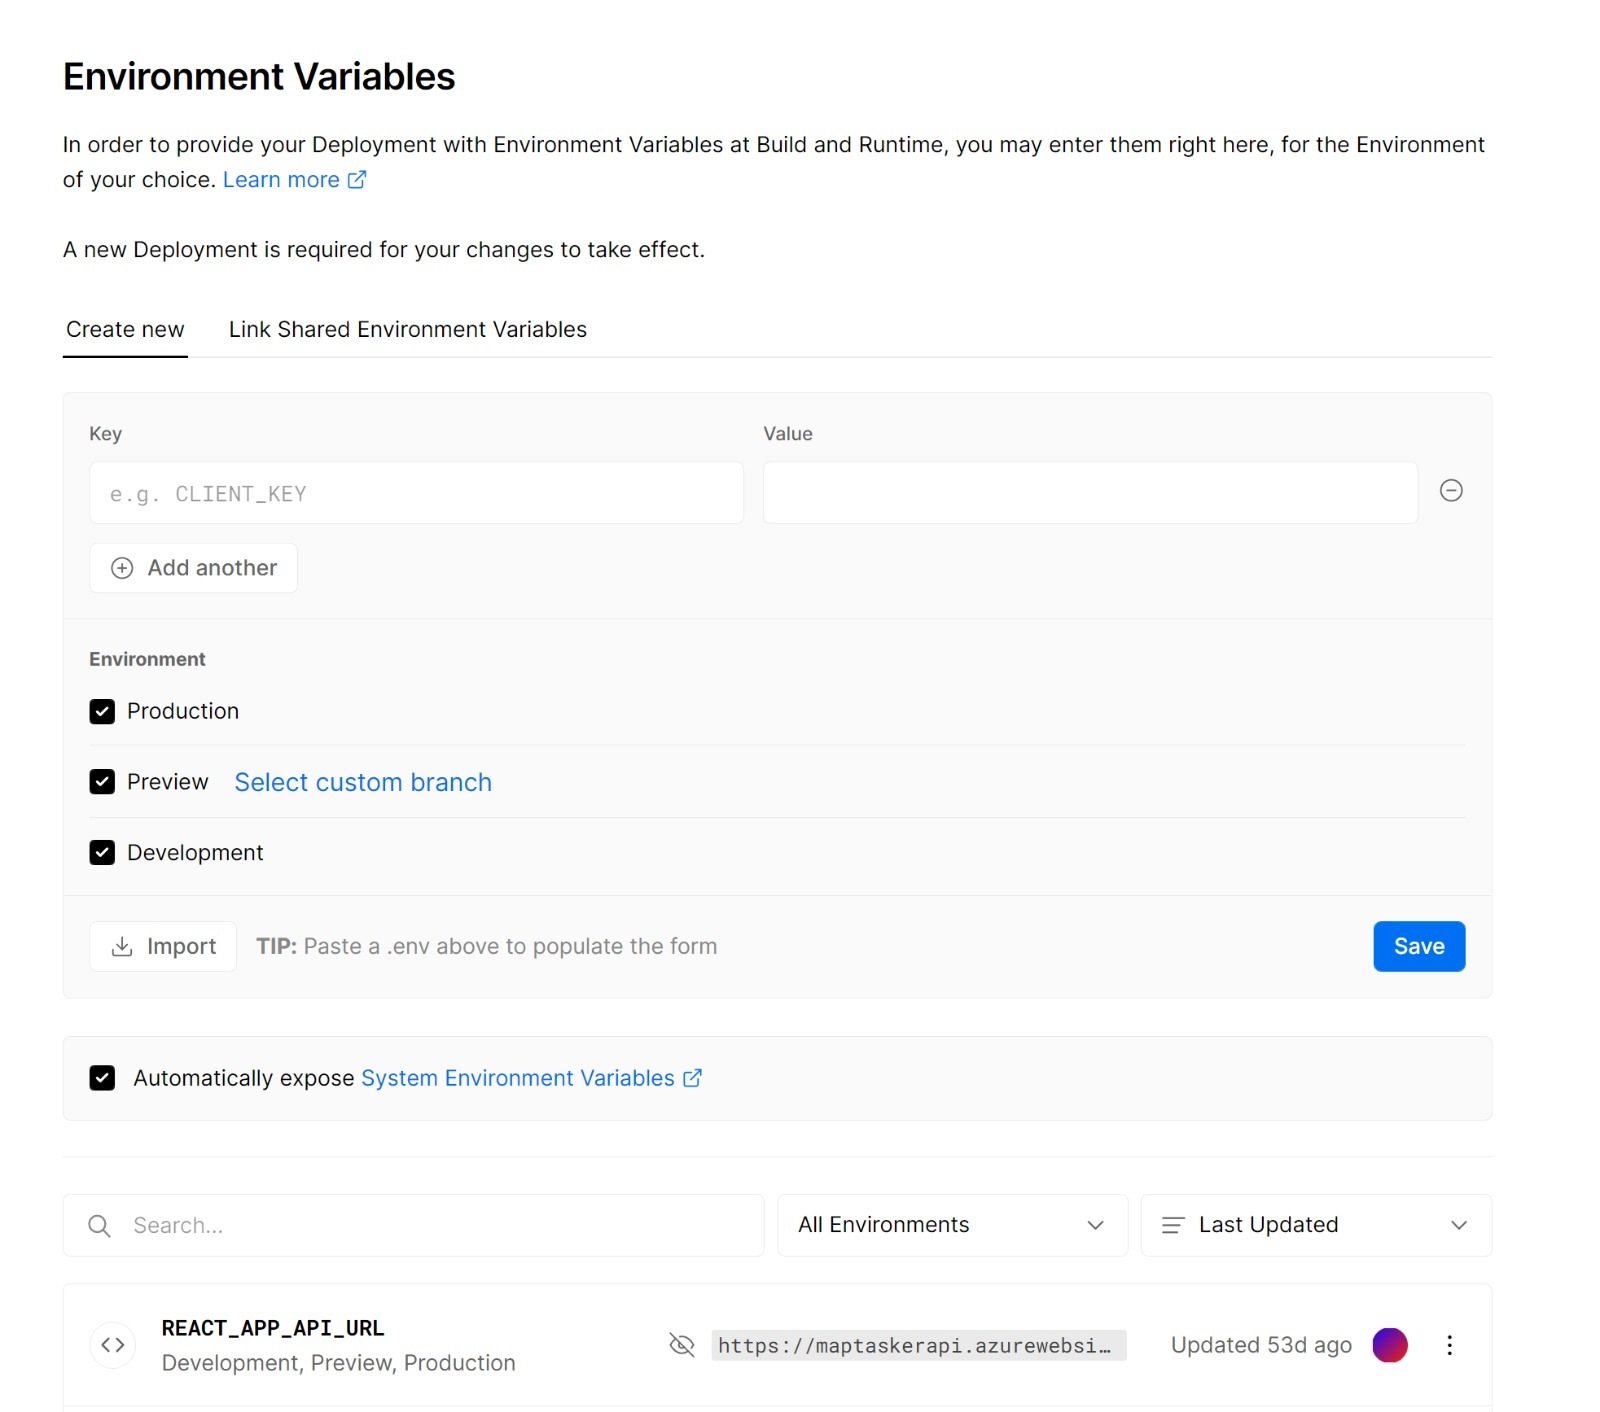
\includegraphics[width=\linewidth]{./slike/front3.jpg}
			  \centering
			  \caption{Podešavanje varijabli okruženja}
		  \end{figure}

		  \vspace{20mm}

		  \noindent Spremanjem postavki razmještanje frontenda će se dogoditi automatski i ponovno se pokrenuti pushanjem na main branch. 
\eject 

